\chapter{Focus Before Diversification}

The exchange begins with an assumption that sounds sensible: perhaps entrepreneurs should diversify beyond one or two things in order to become safer. The answer turns that assumption around. In this School of Hard Knocks interview, curated by LazyingArt LLC, diversification is not first treated as a virtue of maturity. It is treated as a question of sequence: has the founder become strong enough at one business engine to justify spreading attention?

\section{The Question Behind Diversification}

The interviewer asks how important it has been for the speaker, and how important it is for entrepreneurs in general, to diversify beyond just one or two things. That is the natural opening puzzle. More businesses can look like more safety; more sources of income can look like less dependence.

But we have to be careful about what is being diversified. Passive investment capital and founder attention are different objects. A founder is not only allocating money. A founder is allocating judgment, selling time, hiring attention, operational discipline, and the daily force required to make one thing work.

A compact way to mark the distinction is
\begin{equation}
\text{capital spread}
\neq
\text{founder attention spread}.
\end{equation}
This is not board notation from the video; no usable board image was preserved. It is a notation for the argument in the interview. In a financial portfolio, spreading capital may reduce exposure. In an operating company, spreading the founder too early may reduce competence.

\subsection{Question \& Answer}

\paragraph{Question.}
Should entrepreneurs diversify beyond one or two things?

\paragraph{Answer.}
The speaker answers directly: he does not think people should diversify. The point is not that diversification can never be useful. The point is that early diversification can become a way of limiting failures because the founder is not yet great at one thing.

So the first lesson is conditional:
\begin{equation}
\text{early diversification}
\neq
\text{automatic prudence}.
\end{equation}
The question asks about breadth. The answer insists on order.

\section{The Reversal: Focus Before Spread}

The speaker then reaches for an outside formulation, attributed loosely to Mark Cuban or someone similar: diversification is for people who are not great at one thing. The attribution should remain loose, because the interview itself gives it that way. The useful part is the mechanism.

Let \(B_1\) denote the first real business engine. The founder has two very different questions available:
\begin{align}
&\text{How do we become excellent at } B_1? \\
&\text{How do we reduce our exposure to } B_1?
\end{align}
The first question is about mastery. The second is about cushioning. The speaker's warning is that cushioning can arrive before mastery.

That is why the word ``diversification'' can be misleading in an entrepreneurial setting. It may sound like disciplined risk management, but in the early stage it can also mean that the founder is distributing unfinished execution across several fronts.

\section{A Minimal Attention Model}

There is no extracted screenshot containing equations or diagrams for this lecture, so the model here is only a bookkeeping reconstruction of the interview logic. It makes explicit the arithmetic behind the speaker's warning.

Let the founder have one normalized unit of operating attention:
\begin{equation}
A = 1.
\end{equation}
If the founder divides that attention across \(n\) active projects, then the attention per project is
\begin{equation}
a_n = \frac{A}{n} = \frac{1}{n}.
\end{equation}
Now suppose execution quality depends positively on focused attention. Write that quality as \(q(a)\), with the simple monotonic assumption
\begin{equation}
a_1>a_2
\quad \Longrightarrow \quad
q(a_1)>q(a_2).
\end{equation}
For \(n>1\), we have \(1/n<1\), and therefore
\begin{equation}
q\!\left(\frac{1}{n}\right) < q(1).
\end{equation}
This does not prove that every founder should always do one thing. It only formalizes the local claim: if the bottleneck is founder competence and attention, adding more projects can reduce the quality applied to each one.

\paragraph{Worked example.}
Take the simplest illustrative rule,
\begin{equation}
q(a)=a.
\end{equation}
One focused business receives
\begin{equation}
q(1)=1,
\end{equation}
while four simultaneous projects receive
\begin{equation}
q\!\left(\frac{1}{4}\right)=\frac{1}{4}
\end{equation}
per project. The arithmetic captures the spoken mechanism: diversification may look like protection, but it can also spread underdeveloped execution.

\begin{figure}
\centering
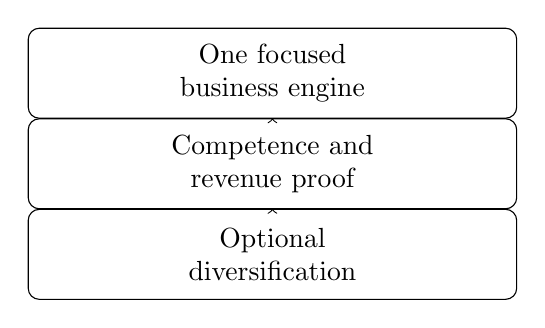
\begin{tikzpicture}
\node[draw, rounded corners, align=center, text width=2.35in, minimum height=0.45in] (focus) at (0,0) {One focused\\business engine};
\node[draw, rounded corners, align=center, text width=2.35in, minimum height=0.45in] (proof) at (0,-1.15) {Competence and\\revenue proof};
\node[draw, rounded corners, align=center, text width=2.35in, minimum height=0.45in] (option) at (0,-2.3) {Optional\\diversification};
\draw[->] (focus) -- (proof);
\draw[->] (proof) -- (option);
\end{tikzpicture}
\caption{A transcript-derived reconstruction of the sequence implied by the interview: focus first, prove the engine, then consider diversification.}
\end{figure}

\section{The Revenue Anecdote}

After the general reversal, the speaker moves into his own chronology: he says he did not start by diversifying. His solar company was already doing more than ten million dollars in revenue.

We can preserve that quantitative anchor as
\begin{equation}
R_{\mathrm{solar}} > 10{,}000{,}000 \ \text{dollars}.
\end{equation}
Here \(R_{\mathrm{solar}}\) denotes the reported revenue of the solar company. This is not a universal rule and not a formal threshold for all founders. It is an anecdotal marker of proof.

The order matters more than the number. Diversification comes after evidence that one commercial engine works:
\begin{equation}
\text{focus}
\longrightarrow
\text{revenue proof}
\longrightarrow
\text{possible expansion}.
\end{equation}
That is the payoff of the answer. The speaker is not merely saying ``do less.'' He is saying that breadth should be earned by depth.

\section{Claim, Anecdote, And Mechanism}

For later chapters in an entrepreneurship book, it is useful to separate the layers of the interview.

\paragraph{Claim.}
The speaker does not think entrepreneurs should diversify early.

\paragraph{Anecdote.}
He says his own diversification did not come first; the solar company had already reached more than ten million dollars in revenue.

\paragraph{Mechanism.}
Premature diversification can limit failures rather than build mastery. It can reduce the pain of being wrong without forcing the founder to become excellent at one thing.

This distinction keeps the chapter source-conscious. The interview gives us a sharp opinion, an uncertain borrowed saying, and a concrete revenue anecdote. It does not give a complete theory of diversification.

\section{Summary}

The lecture begins with diversification as the presumed virtue and answers with focus as the prior discipline. The useful rule is not ``never diversify.'' It is narrower and stronger: do not use diversification as a substitute for becoming good at one commercial engine.

Once the engine has proof, diversification may become optionality. Before proof, it may only distribute weakness.